%!TEX root = ../thesis.tex
\chapter{Introduction}  % Main chapter title
\label{cha:introduction}

%----------------------------------------------------------------------------------------
%	SECTION 1
%----------------------------------------------------------------------------------------

\section{Main Section 1}


MR relation ship image arXiv:1506.05097~\citet{chen_probabilistic_2016}

\begin{figure}
    \centering
    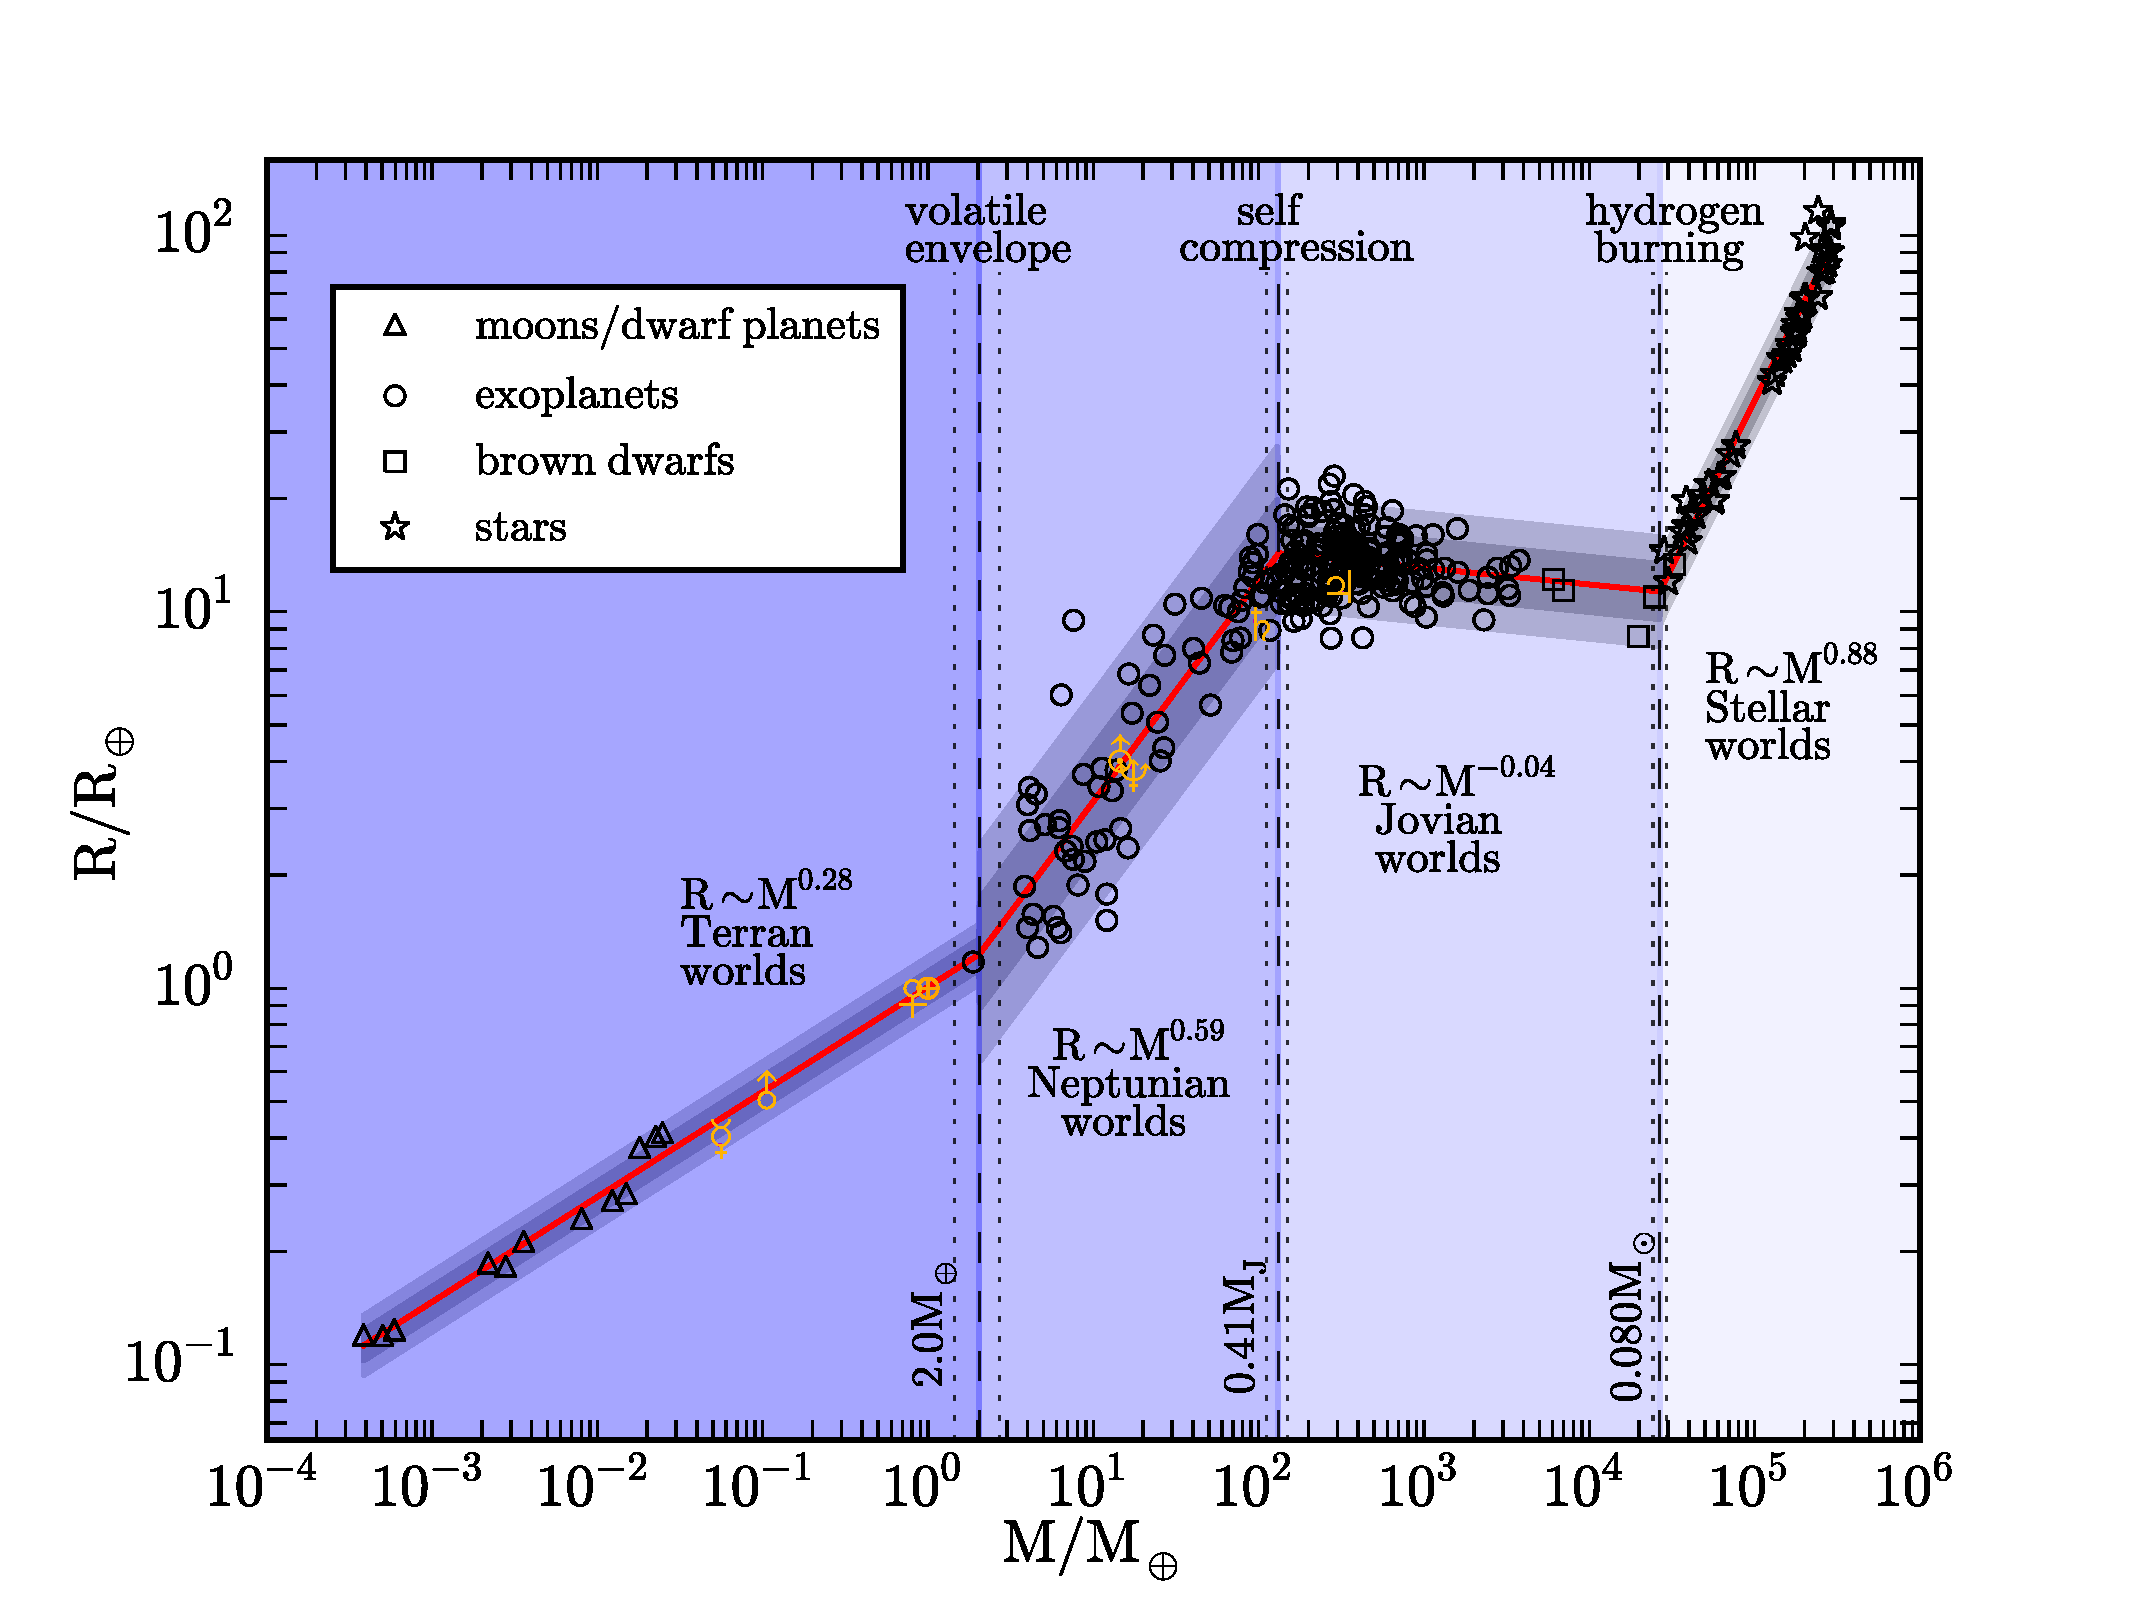
\includegraphics[width=0.7\linewidth]{./figures/introduction/plt_overlay_add.pdf}
    \caption{M-R relationship~\citet{chen_probabilistic_2016}}
    \label{fig:pltoverlayadd}
\end{figure}

Santos et al 2017 \todo{read and quote}

%-----------------------------------
%	SUBSECTION 1
%-----------------------------------
\subsection{Subsection 1}


%-----------------------------------
%	SUBSECTION 2
%-----------------------------------

\subsection{Subsection 2}

%----------------------------------------------------------------------------------------
%	SECTION 2
%----------------------------------------------------------------------------------------

\section{Main Section 2}


Spectral Disentangling techniques
- PSOAP
- Differencing Fruluga
- Templates ?


2D-cross-correlation?   piskorz 2016


\section{Recent detections in Companion spectra.}


Birkby


\subsection{model fitting transit stars (not actual title. more other similar methods)}
There are other situations in which to determine the presence of faint secondary spectra, such as, identifying the presence of any background or companion stars of transiting planet candidates. Many astronomical phenomena such as grazing eclipsing, a giant primary star eclipsed by a dwarf or a background star can produce signals indistinguishable from planetary transits. Efforts to characterize the false positive probability (FPP) among Kepler planet candidates is as high as $\sim35\%$~\citep{santerne_sophie_2012}. The presence of unknown companions or background stars decreases the dimming effect from the planet transit leading to smaller planetary radius. Where multiple stars are present there may also be ambiguity on which star hosts the planet.~\citet{kolbl_detection_2015} developed a method for detecting the presences of faint secondary lines in optical stellar spectra by matching observations to the SpecMatch library of stellar spectra. Identifying the spectroscopic evidence of a secondary star for 63/1160 California \emph{Kepler} Survey objects of Interest (KOI).


For transiting planets that presence of a background star or a companion star causes problems in characterizing the planet. Being able to detect spectra signal of the a faint second spectra in double-lined spectroscopic binaries.
For example eclipsing binaries,
A dim binary system companion or a gaint planet around a background star can mimic the transit of a small Earth-like planet on a foreground star.






\subsection{Earths atmosphere}
While the Earth's atmosphere is important for an Astronomer's lungs, it can be a nuance for their ground-based observations. As light form astronomical sources passes through the atmosphere, its molecular components absorb some of the light, changing spectral components observed  by imprinting a transmission spectrum of our atmosphere. The H20 absorption is a key example as it defines the photometric and spectroscopic bands in the NIR. \missingfigure{example to point to}.

The correction of observations from the contamination of Earth's atmosphere is a complex process. The transmission is variable on many different time scales, the water vapour change is rapid, concentrations of atmospheric constituents, to seasonal and longer. Such as the increase in atmospheric CO2 causing anthropamorphic climate change this requires 6\% change to C02 line depths since 2000 Molecfit paper? There is also variation with airmass, which depends on the observation angle in the sky and changes as targets move across the sky during the night. 

other constituents, Co Co2 CH4 ..., angle of observations.

An important consideration in the detecting the constituents of planetary atmospheres is the characterization and removal of Earths telluric lines.

e.g. 50\% error in CO2 detection on Mars atmosphere


Recently \citet{Ulmer-moll} compared the telluric correction possible from three different synthetic telluric software agaisnt the standard star model. Molecfit, a software from ESO was the most .

This is a growing field and there are other software available too... 


Water vapour content has rapid variablility. Works such as Snellen 2011, ... ...  model the telluric variation during a observations to remove telluric lines and detect planetary lines.

\todo{finish this}